
% Background Chapter
%%%
% New organisation:
%
% Introduction and Literature Review
%   Tropospheric ozone and air quality . . . . .
%   Isoprene and other VOCs . . . . . . . . . . .
%   Formaldehyde (HCHO) . . . . . . . . . . . .
%   Models . . . . . . . . . . . . . . . . . . . . .
%   Aims?
%%%%%%
\chapter{Introduction and Literature Review} % Chapter Title
\label{LR}
  
\section{Tropospheric ozone and air quality}
  \label{LR:O3andAQ}
  \subsection{Air Quality}
    \label{LR:O3andAQ:AQ}
    %%% AUSTRALIA
    
    % Moved to intro    
    
    \subsubsection{Ozone}
      %%% OZONE
      
      
      
    
    \subsubsection{Particulate matter and SOA}
      
    
    
    \subsubsection{Factors influencing ozone and PM}
      %\label{LR:O3andAQ:AQfactors}
      
    \subsubsection{How do we measure air quality?}
      
      
      
      
      
  \subsection{Ozone transported from the stratosphere}
    
    
    
    
    
    
    
    
  

  \subsection{Ozone formed in the troposphere}
    \label{LR:O3andAQ:BiogenicOzonePrecursors}
    
    
    
\section{Hydroxyl (OH) and other radicals}
  \label{LR:Radicals}
  
  
  
  
  

\section{Isoprene and other VOCs}
  \label{LR:VOCs}
  \subsection{What are VOCs}
    

    
  \subsection{What do they Do?}
    
    
    
  \subsection{Isoprene Cascade}
  
    
  \subsection{How and where do we measure them?}
    

  
  
  \subsection{Emissions estimates}
    \label{LR:VOCs:EmissionsEstimates}
    
    
  
\section{Formaldehyde (HCHO)}
  \label{LR:HCHO}
  
  %Paragraphs moved to Intro
  \subsection{How HCHO is measured}
  
  \subsection{Satellite Inversion}
  
  \subsection{Satellite HCHO detection}
    \label{LR:HCHO:SatelliteDetection}
    TODO: Refactor this section so it's readable
     
    
      
    
    
    \subsubsection{Satellite uncertainties}
      
    
    
  \subsection{Glyoxyl TODO: move somewhere fitting?}
  
    Another chemical retrievable from satellite observation is Glyoxyl, which can be used to further determine what sort of precursors to HCHO are being emitted \citep{Stavrakou2009, Miller2014, Miller2017}.
    TODO: go through 2014 paper and see if it's easy to retrieve, then email Dr. Chris Miller.
    For example \cite{Cao2018_discuss} recently used Glyoxyl measurements to improve understanding of biogenic and anthropogenic NMVOC emissions over China.
    This involved using a method pioneered by \cite{Stavrakou2009} TODO: get this cite and check method out.
   
    Glyoxyl (CHOCHO) is important to us as it shares many properties with HCHO, and may provide additional information in determining isoprene emissions.
    Glyoxyl is another product of VOC oxidation in the atmosphere, with isoprene being the main source globally.
    Under high NO$_X$ conditions, glyoxyl forms rapidly, similarly to HCHO.
    However, glyoxyl also forms in low NO$_X$ environments both slowly (through isoprene epoxydiols), and rapidly (through di-hydroperoxide dicarbonyl compound photolysation \citep{Crounse2013}.
    This process is similar to the proposed mechanisms for hydroperoxyaldehydes by \cite{Peeters2014} and carbonyl nitrates \citep{Muller2014}.
    Aromatics which are largely anthropogenic form glyoxyl quickly, while HCHO is produced slower, allowing determination of anthropogenic sources \citep{Cao2018_discuss}.
    
    HCHO has been used to estimate isoprene emissions (some examples in Section \ref{LR:HCHO:SatelliteInversion}) but many uncertainties exist.
    One of these uncertainties is the yield of HCHO from isoprene, especially in low NO$_X$ environments.
    Glyoxyl could prove complementary to HCHO in constraining isoprene emissions (TODO: Read and cite Vrekoussis2009,2010, Chan Miller 2014, Alvarado 2014) \citep{Miller2017}.
    Recently \cite{Miller2017} updated GEOS-Chem to include the prompt formation of glyoxyl and compared this with satellite and airplane measurements over the USA.
    Glyoxyl is formed by isoprene oxidation rapidly in low NO$_X$ conditions, unlike HCHO.
    With coming geostationary satellites, which provide greater time resolved measurements of HCHO and CHOCHO, this mechanism could be used to clearly show when low NO$_X$ isoprene chemistry is being undertaken \citep{Miller2017}.
    
\section{Models}
  \label{LR:Models}
  \subsection{How can models help}
    
    Models can fill the gaps (both spatial and temporal) in measurement records, and are used to predict/avoid/mitigate hazardous scenarios.
    They are used ideally to steer us away from unsustainable pollution and help complete our understanding of the world from small to large scales.
    They can be used to increase measurement accuracy (for instance in satellite measurements) and determine where we lack information, while also checking the performance of new instruments.
    Precisely representing various chemicals and reactions in the atmosphere allows efficient mitigation of pollution, since we can compare scenarios against one another.
    Currently, improved isoprene understanding is critical for effective air quality measuring \citep{Marvin2017}.
    
    Chemical Transport Models (CTMs) simulate production, loss, and transport of chemical species.
    This is generally calculated using one or both of the Eulerian (box) or Lagrangian (puff) frames of reference.
    CTMs normally solve the continuity equations simultaneously with chemical production and loss for chemicals under inspection. 
    The continuity equations describe transport of a conserved quantity such as mass, which, solved together with production and loss of a chemical can provide detailed simulations of natural processes.
    Models provide a simulation of chemical densities and transport over time as a model runs.
    The general continuity equation links a quantity of a substance (q) to the field in which it flows and can be described by the formula:
    \begin{eqnarray*}
      \frac{\partial \rho}{\partial t} + \nabla \cdot j &=& \sigma 
    \end{eqnarray*}
    where $\rho$ is density of q in the field, t is time, $\nabla$ is divergence, j is the flux (q per unit area per unit time entering or leaving the field), and $\sigma$ is the generation or loss of q per unit volume per unit time.
    
    
    The type of model best suited to modelling the entire earth uses the Eulerian frame of reference, where the atmosphere is broken up into 3-D boxes with densities and transport calculated and stored for sequential steps in time at each location.
    The mass balance equation must be satisfied in any realistic long term box model and is as follows: 
    \begin{align*}
      \frac{dm}{dt} &=& \sum{sources}-\sum{sinks} \\
      &=& F_{in} + E + P - F_{out} - L - D 
    \end{align*}
    where m is mass of a chemical, E and D are emission and deposition, P and L are production and loss, and F is chemical transport in and out, as shown in figure \ref{LR:Models:fig_boxmodel}.
    Many chemical species interact with each other through production and loss. 
    Any large chemical model will solve this mass balance equation over highly coupled arrays of partial differential equations which can be complex and time consuming.
    
    \begin{figure}
      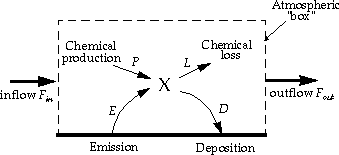
\includegraphics{Figures/boxmodel.png}
      \caption{ %
        Standard box model parameters, image taken from \cite{Jacob_1999_book}. }
      \label{LR:Models:fig_boxmodel}
    \end{figure}
    
    In many CTMs the isoprene emissions are calculated seperately using MEGAN, and then used as boundary conditions (EG: \cite{Guenther2006}). 
    This can speed up calculations as the transport and concentrations can be simulated in various conditions without recalculating the emissions.
    Trace gases with short lifetimes and complex chemistry such as isoprene are often hard to measure which makes verifying model estimates difficult.
    Contemporary models generally use mathematical differential solving tools of various complexity to solve chemical equations and reaction rates (often called chemical mechanisms) in order to predict an environments evolution over time.
    Different solvers may be slower or faster and more suited to particular situations based on the stability of the equations and systems involved, and chemical mechanisms may vary in how many reactions and chemicals are listed and grouped together.
    For example: Since [O] $<<$ [O$_3$] the chemical family O$_X$ (  O$_X \equiv $ O $+$ O$_3$ ) can be used to simplify chemistry simulations and approximate O$_3$ concentrations \citep[][Chapter 3]{BrasseurJacob2017}.
    \cite{Zhang2012} examine the outputs from a regional model (WRF/Chem) using three different chemical mechanisms, and they show that particulate matter prediction is sensitive to the choice of chemical mechanism. 
    
  \subsection{Relevant model frameworks}
  \label{LR:Models:frames}
    
    % Outline of ACM
    Atmospheric chemistry models (ACMs) require various inputs and can be sensitive to ozone and oxidative parameterisations. 
    TODO: read more Christian 2017,
    TODO: put some more generic ACM info here.
    
    \subsubsection{Box models} 
    \label{LR:Models:frames:box}
    % for example CAABA/MECCA
      A box model involves modelling chemistry in a singular set of conditions without transport or any spatial gradients.
      One box model used in this thesis is called CAABA/MECCA, and is described here as an example.
      
      CAABA (Chemistry As A Boxmodel Application) estimates the chemical concentrations accounting for J-values (JVAL), simplified and parameterised photolysis (SAPPHO) and simplified emission and depositions (SEMIDEP).
      CAABA runs in a single scenario (or box) with given emissions, depositions, and initial concentrations, allowing the examination of chemistry in a very specific environment to be modelled with high temporal resolution.
      This has been used with an atmospheric chemistry model MECCA (Module Efficiently Calculating the Chemistry of the Atmosphere) which implements tropospheric and stratospheric chemistry for both the gas and the aqueous phases \citep{Sander2005}.
      MECCA chemical mechanisms include basic O$_3$, CH$_4$, NO$_X$, and HO$_X$ chemistry, as well as non methane hydrocarbon (NMHC) chemistry, considering gas phase, aqueus phase, and heterogenous reactions. \citep{Sander2005}
      For the numerical integration, MECCA uses the KPP software (\cite{SanduSander2006}), which takes chemical reactions and their rate coefficients and codes integral solutions to the system.
      The combination of the CAABA box model with MECCA module is called CAABA/MECCA and is currently at version 3.
      CAABA/MECCA been implemented for various calculations including ozone chemistry throughout the atmosphere in \cite{Zanis2014}.
  
      MECCA could also be used as the chemistry mechanism for a more complex, 3-dimensional model (\cite[e.g.][]{Jockel2006}).
      The connection is established via the MESSy interface (\url{http://www.messy-interface.org}) developed by \cite{Jockel2005} as part of an effort to simplify the framework for modelling the atmospheres at various scales.
      The user manual is available online at \url{http://www.rolf-sander.net/messy/mecca/caaba_mecca_manual.pdf}.
  
      By allowing for interactions between boxes this concept can be extended to multiple-box models.
      These are simply multiple instances of single boxes with the addition of transport between them, which generally requires a meteorological model to provide winds, and other transport mechanisms.
      
    \subsubsection{Chemical transport} %% eg. GEOS-Chem
      GEOS-Chem is an example of this, with many boxes covering the globe, each with chemistry and dynamic meteorological conditions.
      The transport between boxes also needs to be taken into account when simulating concentrations.
      Additionally the different meteorological conditions such as wind and air pressure need to be handled within each box.      
      GEOS-Chem has a meteorological model coupled to a chemical model, which simulates the world in a three dimensional grid of connected boxes.
      
      GEOS-Chem is a well supported global, Eulerian CTM with a state of the science chemical mechanism, with transport driven by meteorological input from the Goddard Earth Observing System (GEOS) of the NASA Global Modeling and Assimilation Office (GMAO).
      GEOS-Chem simulates more than 100 chemical species from the earth's surface up to the edge of space (0.01~hPa) and can be used in combination with remote and in-situ sensing data to give a verifiable estimate of atmospheric gases and aerosols.
      It was developed, and is maintained, by Harvard University staff as well as users and researchers worldwide.
      Several driving meteorological fields exist with different resolutions, the finest at 0.25 by 0.3125$^\circ$ horizontally at 5 minute time steps with 72 vertical levels.
      
      Global CTMs are often run using one or several emission models (or the output from them) to determine boundary conditions for many gridboxes.
      TODO: is this the case? Doesn't GEOS-Chem have coupled chemistry and meteorology? Check the wiki.
      GEOS-Chem has boundary conditions based on several meteorological and emissions inventories, the following are the versions of theses used by GEOS-Chem v 10.01. 
      Meteorological fields can be driven by NASA's GEOS-5 data (0.5$^{\circ}$ x 0.666$^{\circ}$) \citep{Chen2009}, which exists up to 2013, or GEOS-FP data (0.25$^{\circ}$ x 0.3125$^{\circ}$).
      Fire emissions come from the GFED4 product \citep{Giglio2013}. 
      Anthropogenic VOC emissions come from the EDGAR inventory, while biogenic VOC emissions are coupled to the MEGAN model TODO:cites.
      The estimated biogenic VOC emissions are important for accurately simulating chemistry within models, as discussed in Sections \ref{LR:O3andAQ:BiogenicOzonePrecursors} and \ref{LR:Models:Unc}.
      
      The Model of Emissions of Gases and Aerosols in Nature (MEGAN) is one of the more commonly used natural emission models \citep{Monks2015}. (TODO: more cites which say this/use MEGAN)
    
    \subsubsection{Land based emissions} %% EG MEGAN
      % TODO: Overview of land based emissions modelling?
      
      MEGAN is a global model with resolution of around 1~km, and is used to generate the BVOC emissions used in various global chemistry models such as GEOS-Chem.
      MEGAN uses leaf area index, global meteorological data, and plant functional types (PFTs) to simulate terrestrial isoprene emissions.
      The model includes global measurements of leaf area index, plant functional type, and photosynthetic photon flux density, from remote sensing databases \citep{Kefauver2014}.
      The various PFTs are used to generate emission factors which represent quantities of a compound released to the atmosphere through an associated activity.
      For example, an emission factor for isoprene within a forest would include the requirement of sunshine and suitable temperature.
      The schematic for MEGAN, taken from \citet{Megan_Website}, is shown in figure \ref{LR:models:frames:fig_megan_schematic}
      
      \begin{figure}[!htbp]
        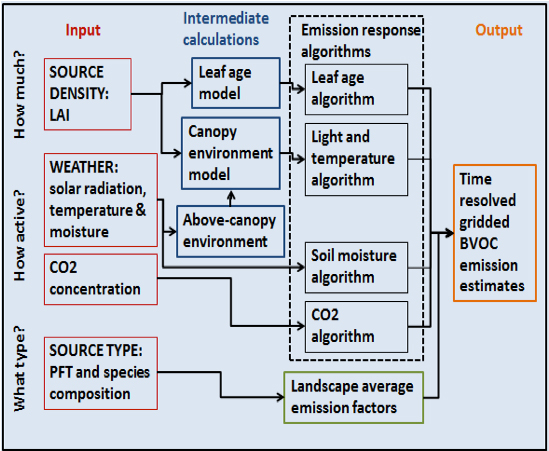
\includegraphics[width=\textwidth]{Figures/MEGANmodel_img.jpg}
        \caption{MEGAN schematic, copied from \citet{Megan_Website}}
        \label{LR:models:frames:fig_megan_schematic}
      \end{figure}
      
      MEGAN ``is a modelling framework for estimating fluxes of biogenic compounds between terrestrial ecosystems and the atmosphere to account for the major known processes controlling biogenic emissions.'' \citep{Guenther2012}.
      It allows parameterisation of various BVOC emissions, with descriptions given in \cite{Guenther2012}.
      Instructions to run version 2.1 are available at \url{http://lar.wsu.edu/megan/docs/MEGAN2.1_User_GuideWSU.pdf}, and a version using the Community Land Model (CLM) is available at \url{http://www.cesm.ucar.edu}.
      It uses meteorological fields from the Weather Research and Forecasting (WRF) modelling system.
      Version 2.1 (updated from 2.0 \citep{Guenther2006}) includes 147 species, in 19 BVOC classes, which can be lumped together to provide appropriate output for mechanisms in various chemical models.
      
      MEGAN was developed as a replacement for two earlier canopy-environment emission models (BIES and GEIA), and initially included a simple canopy radiative transfer model, which parameterised sun-lit and shaded conditions through a canopy.
      Early models didn't account for abiotic stresses, such as drought, prior rainfall and development processes, although these influenced species specific emissions by more than an order of magnitude \citep{Niinemets1999}.
      Isoprene emissions were based on temperature, leaf area, and light, but have since been updated to include leaf age activity \citep{Guenther2000}, and a leaf energy balance model \citep{Guenther2006} in MEGANv2.0.
      This update included a parameter for soil moisture, to account for drought conditions, however this parameter is currently (as of version 2.1) not applied to isoprene \citep{Sindelarova2014}.
      Soil moisture effects on isoprene emission are very important, and can drastically affect estimates.
      
      MEGAN has recently been analysed using 30 years of meteorological reanalysis information by \cite{Sindelarova2014}.
      They estimate emissions of Biogenic VOCs (BVOCs) to be 760~Tg(C)yr$^{-1}$, 70\% (532~Tg(C)yr$^{-1}$) of which is isoprene.
      This is similar to isoprene emission estimates from MEGAN itself, of 400-600~Tg(C)yr$^{-1}$ \citep{Guenther2006}.
      MEGAN emissions estimates are termed bottom-up, as opposed to top-down which are derived from satellite measurements of the products of various VOCs.
      Using GOME satellite HCHO and a Beyesian inversion technique to derive isoprene emissions, \cite{Shim2005} estimated global isoprene emissions to be $\sim566$~TgC yr$^{-1}$. 
      This estimate is greater than initially thought and leads to decreased ($\sim10\%$) simulated OH concentrations to 9.5e5 molec cm$^{-3}$.
      
      Improvements to emissions models require improved understanding of regions and their behaviour.
      Inaccuracies can arise due to lack of data, such as the large and sparsely measured Australian outback.
      MEGAN has been shown to overpredict isoprene and underpredict monoterpene emissions in southeast Australia, with peaks and troughs captured but not at the right magnitude (\cite{Emmerson2016}).
      MEGAN output in Australia is adversely affected by poor emission factor estimation. 
      An example can be seen in \citet{Muller2008} where MEGAN overestimates isoprene in northern Australia.
      Underestimates of monoterpenes may be due simply to underestimated emission rates for many Eucalypt species \citep{Winters2009}.
      

    \subsubsection{Radiative transfer} %% EG LIDORT
      %TODO: Lidort example?
      TODO: Lidort example?
    
  \subsection{Factors affecting isoprene emissions estimates}

      \cite{Marais2014} examine factors affecting isoprene emissions, showing how emissions are sensitive to various environmental factors.
      Their work used MEGAN \citep{Guenther1995} and GEOS-Chem to look at how these factors affect surface ozone and particulate matter in Africa.
      One of the important uncertainties seen in MEGAN within this work is the isoprene emissions due to plant type.
      Canopy level isoprene measurements are made using relaxed eddy accumulation (REA) at several sites in Africa.
      One plant type near a measurement site emits more than other species and it's actual distribution on a larger scale is completely unknown - leading to possible overestimations in MEGAN.
      Current emissions estimates require more validation against observations, and recently a comparison of two major VOC models (MEGAN and ORCHIDEE) was undertaken by \cite{Messina2016} reiterating this requirement.
      In their work they examine model sensitivities and show that the important parameters are leaf area index (LAI), emission factors (EF), plant functional type (PFT), and light density fraction (LDF).
      There is high uncertainty in LAI and EF, which require more or improved measurements at the global scale.
      LDF paramterisation needs improvement and these models require more PFTs.
      Global emissions inventories like MEGAN suffer from large extrapolations which introduce uncertainties \citep{Miller2014}.

      \cite{Emmerson2016} analyse EF sensitivity of a high resolution model of atmospheric chemistry over southeast Australia, comparing isoprene and monoterpene emissions against 4 separate campaigns.
      They show that the effect on total emissions is roughly linear and that no blanket EF changes are appropriate for all regions/seasons.
      They also mention that Australian eucalypt emissions are based on samples from young trees, which may emit more isoprene than older trees.
      
      \cite{Stavrakou2014} examined modelled Asian emissions and altered model parameters for temperature, plant type emission factors, incoming solar radiation (insolation) intensity, land use changes, and palm tree forest expansion.
      Changes were constrained by a network of radiation measurements and some experiments with south east Asian forest emissions - and led to reduction in isoprene emissions by a factor of two over the region.
      The Asian region is also shown to have a strong correlation with the Oceanic Niño Index (ONI), with positive anomalies associated with El Niño.
      In the last 20 years anthropogenic emissions of VOCs have been increasing while biogenic VOC emissions have decreased due to rapid economic growth and lower annual temperatures \citep{Stavrakou2014, Kwon2017}.
      
      %Temperature has a strong exponential relationship with isoprene emissions, and can be readily seen in comparisons to a major isoprene product HCHO. 
  
  % TODO: Reading up to here
  \subsection{Uncertainties}
    \label{LR:Models:Unc}
    Here I will attempt to list and partially explain the major uncertainties models have in relation to  VOCs, SOAs, and ozone. 
    TODO: Is this a good idea or should I put any pertinent uncertainties with the associated work/descriptions?
    
    \subsubsection{Emissions Inventories}
      % Emissions Inventories 
      Using different emissions inventories in an ACM can have large impacts on the simulation.
      Natural (biogenic or pyrogenic) and human driven (anthropogenic) emissions often drive a large fraction of atmospheric oxidation and radical chemistry, especially in the continental boundary layer.
      \cite{Zeng2015} examine the affects on CO and HCHO when running simulations with two different inventories.
      TODO: find where I took notes about Zeng2015 and put them here.
    
    %% GEOS-Chem resolution uncertainties
    \subsubsection{Resolution}
      \label{LR:Models:Unc:Resolution}
      GEOS-Chem simulations are somewhat sensitive to the resolution at which you run.
      For example: \cite{Wild2006} show that reduced resolution increases OH concentrations and ozone production rates.
      \cite{Christian2017} find small changes in OH ($<10$\%) in OH, HO$_2$ and ozone concentrations local to the north american arctic, when changing from 4 by 5 to 2 by 2.5\degr resolution, however they continue at lower resolution to save computational time.
      
      For many global scale analyses, errors from resolution are less important than those from chemistry, meteorology, and emissions (\cite{Christian2017}).
      
    
    % Transport uncertainties?
    \subsubsection{Transport}
      \label{LR:Models:Unc:Transport}
      TODO: Literature showing transport uncertainties or lack thereof     
      %TODO: examples of transport uncertainties
    
    \subsubsection{Chemistry mechanisms}
      \label{LR:Models:Unc:Chemistry}
      %% GEOS-Chem Ozone uncertainties 
      There is still much work to be done in models to correctly simulate the various precursors to HCHO.
      Often HCHO is used as a way of checking if these precursors are correctly modelled since HCHO measurements are more readily available (for instance from satellites).
      GEOS-Chem has recently been analysed for sensitivity for ozone along with oxidants (OH and HO$_2$) \citep{Christian2017}.
      \cite{Christian2017} found that GEOS-Chem ozone was most sensitive to NO$_2$ photolysis, the $NO_2 + OH$ reaction rate, and various emissions.
      They used GEOS-Chem v9-02, with $4^{\circ} \times 5^{\circ}$ resolution, and while the low resolution adds errors in OH concentrations and O$_3$ production rates, the errors from chemistry, meteorology, and emissions are much larger.

      \cite{Marvin2017} suggest that isoprene mechanisms in several contemporary models (including GEOS-Chem) are inadequate. 
      They show that for a specific measurement campaign, the HCHO concentrations are underestimated in a way that can not be easily fixed through rate constant changes.
      Recently \cite{Marvin2017} compared five global ACMs isoprene mechanisms by evaluating simulated HCHO mixing ratios compared to in situ measurements from the Southeast Nexus (SENEX) aircraft campaign (in southeastern USA).
      They compared five models (GEOS-Chem, CB05, CB6r2, MCMv3.2, and MCMv3.3.1) and found all of them underestimated the HCHO concentrations (by $15 - 30\%$).
    
    \subsubsection{Clouds}
      \label{LR:Models:Unc:Clouds}
      One of the major uncertainties in chemical, climate, radiation, and weather models is cloud formation and dynamics.
      Clouds are remarkably complex at a much finer scale than can be accurately modelled by global chemistry models (with current processing power).
      Globally over half (50-60\%) of the world is covered by clouds, with $\sim10\%$ of them being rain-clouds \citep{Kanakidou2005}.
      Wet scavenging performed in clouds not only depends on large scale cloud processes, but also on the microphysics of aerosols being scavenged, differing between aerosol sizes and hygroscopic properties.
      
    \subsubsection{Soil Moisture}
      \label{LR:Models:Unc:SoilMoisture}
      Australia has a unique climate, along with soil moisture, clay content and other important properties which affect VOC emissions.
      These properties are poorly understood in Australia due to the continents size and the relative sparsity of population centres, which make many areas very difficult or expensive to reach.
      Soil moisture plays an important role in VOC emissions, as trees under stress may stop emitting various chemicals. 
      This is especially true for Australia due to frequent droughts and wildfires.
      The argument for improved understanding of land surface properties, specifically soil moisture, is an old one\citep{Mintz1982, Rowntree1983, Chen2001}. 
      \cite{Rowntree1983} show how quickly soil moisture anomalies affect rainfall and other weather systems, while \cite{Chen2001} specifically show how important fine scale soil moisture information is when modelling land surface heat flux, and energy balances.
      Modelled emissions are sensitive to soil moisture, especially near the soil moisture threshold (or wilting point), below which trees stop emitting isoprene and other VOCs completely as they can no longer draw water \citep{Bauwens2016}.
      MEGAN accounts for soil moisture by applying it as an emission factor (EF) which scales the emission rate of various species.
      \cite{Sindelarova2014} show reductions in modelled Australian isoprene emissions of 50\% when incorporating soil moisture in MEGAN estimates. 
      
      Droughts affects can be difficult to measure, as it is a multi-scale problem which affects various aspects of the land-air interface including plant emissions and dry deposition (\cite{Wang2017}).
      The Standardised Precipitation Evapotranspiration Index (SPEI) is a measure of drought using TODO \cite{SPEI_website}.
      This product covers 1901 - 2011, and uses the average over that period as the background, in order to compare drought stressed regions against those with sufficient or excess water \cite{SPEI_website}.
      
